%%%%%%%%%%%%%%%%%%%%%%%%%%%%%%%%%%%%%%%%%
% a0poster Landscape Poster
% LaTeX Template
% Version 1.0 (22/06/13)
%
% The a0poster class was created by:
% Gerlinde Kettl and Matthias Weiser (tex@kettl.de)
%
% This template has been downloaded from:
% http://www.LaTeXTemplates.com
%
% License:
% CC BY-NC-SA 3.0 (http://creativecommons.org/licenses/by-nc-sa/3.0/)
%
%%%%%%%%%%%%%%%%%%%%%%%%%%%%%%%%%%%%%%%%%

%-------------------------------------------------------------------------------
%	PACKAGES AND OTHER DOCUMENT CONFIGURATIONS
%-------------------------------------------------------------------------------

\documentclass[a0, landscape]{a0poster}

\usepackage{multicol} % This is so we can have multiple columns of text side-by-side
\columnsep=100pt % This is the amount of white space between the columns in the poster
\columnseprule=3pt % This is the thickness of the black line between the columns in the poster

\usepackage[svgnames]{xcolor} % Specify colors by their 'svgnames', for a full list of all colors available see here: http://www.latextemplates.com/svgnames-colors

%\usepackage{times} % Use the times font
% \usepackage{palatino} % Uncomment to use the Palatino font
\usepackage{fontspec}
\setmainfont{Latin Modern Sans}

\usepackage{graphicx} % Required for including images
\graphicspath{{figures/}} % Location of the graphics files
\usepackage{booktabs} % Top and bottom rules for table
\usepackage[font=small,labelfont=bf]{caption} % Required for specifying captions to tables and figures
\usepackage{amsfonts, amsmath, amsthm, amssymb} % For math fonts, symbols and environments
\usepackage{wrapfig} % Allows wrapping text around tables and figures
\usepackage[export]{adjustbox}% http://ctan.org/pkg/adjustbox

\usepackage{listings}
\usepackage{color}
\usepackage{mathtools}

\newenvironment{Figure}
  {\par\medskip\noindent\minipage{\linewidth}}
  {\endminipage\par\medskip}

\DeclarePairedDelimiterX{\norm}[1]{\lVert}{\rVert}{#1}
\DeclareMathOperator{\Tr}{Tr}

\definecolor{dkgreen}{rgb}{0,0.6,0}
\definecolor{gray}{rgb}{0.5,0.5,0.5}
\definecolor{mauve}{rgb}{0.58,0,0.82}

\lstset{
  %frame=tb,
  language=Python,
  aboveskip=2mm,
  belowskip=0mm,
  showstringspaces=false,
  columns=flexible,
  basicstyle={\small\ttfamily},
  numbers=none,
  numberstyle=\tiny\color{gray},
  keywordstyle=\color{blue},
  commentstyle=\color{dkgreen},
  stringstyle=\color{mauve},
  breaklines=true,
  breakatwhitespace=true,
  tabsize=3,
  framexleftmargin=15pt
  }


\begin{document}

%----------------------------------------------------------------------------------------
%	POSTER HEADER
%----------------------------------------------------------------------------------------

% The header is divided into three boxes:
% The first is 55% wide and houses the title, subtitle, names and university/organization
% The second is 25% wide and houses contact information
% The third is 19% wide and houses a logo for your university/organization or a photo of you
% The widths of these boxes can be easily edited to accommodate your content as you see fit

\begin{minipage}[b]{0.878\linewidth}
\Large ~Poster W763\\

\veryHuge \color{NavyBlue} \textbf{Multidimensional analysis and detection of informative features in diffusion MRI} \color{Black}\\ % Title
%\Huge\textit{A really awesome subtitle}\\[1cm] % Subtitle
\huge \textbf{Adam Richie-Halford\textsuperscript{1} \& Ariel Rokem\textsuperscript{2}}\\ % Author(s)
\Large 1. Dept. of Physics, 2. The eScience Institute, Univ. of Washington, % University/organization
\Large Contact: \texttt{richford@uw.edu}
\end{minipage}
%
%\begin{minipage}[b]{0.25\linewidth}
%\color{DarkSlateGray}\Large \textbf{Contact Information:}\\
%Department Name\\ % Address
%University Name\\
%123 Broadway, State, Country\\\\
%Phone: +1 (000) 111 1111\\ % Phone number
%Email: \texttt{john@LaTeXTemplates.com}\\ % Email address
%\end{minipage}
%
\begin{minipage}[b]{0.12\linewidth}

\includegraphics[width=9cm]{UWlogo.png}
\end{minipage}

% \vspace{0.5cm} % A bit of extra whitespace between the header and poster content

%----------------------------------------------------------------------------------------

\begin{multicols}{3} % This is how many columns your poster will be broken into, a poster with many figures may benefit from less columns whereas a text-heavy poster benefits from more

%----------------------------------------------------------------------------
%	Introduction
%----------------------------------------------------------------------------

\section*{Introduction to white matter tractometry}

\noindent White matter structure is important to normal brain function. Diffusion tensor imaging (DTI) measures the white matter \emph{in vivo} by fitting a diffusion ellipsoid in every voxel. One of the challenges of DTI is to make sense of the massive dimensionality of the data. One common approach is to reduce the dimensionality of each diffusion tensor to scalars such as mean diffusivity (MD) and fractional anisotropy (FA).
\begin{Figure}
    \centering
    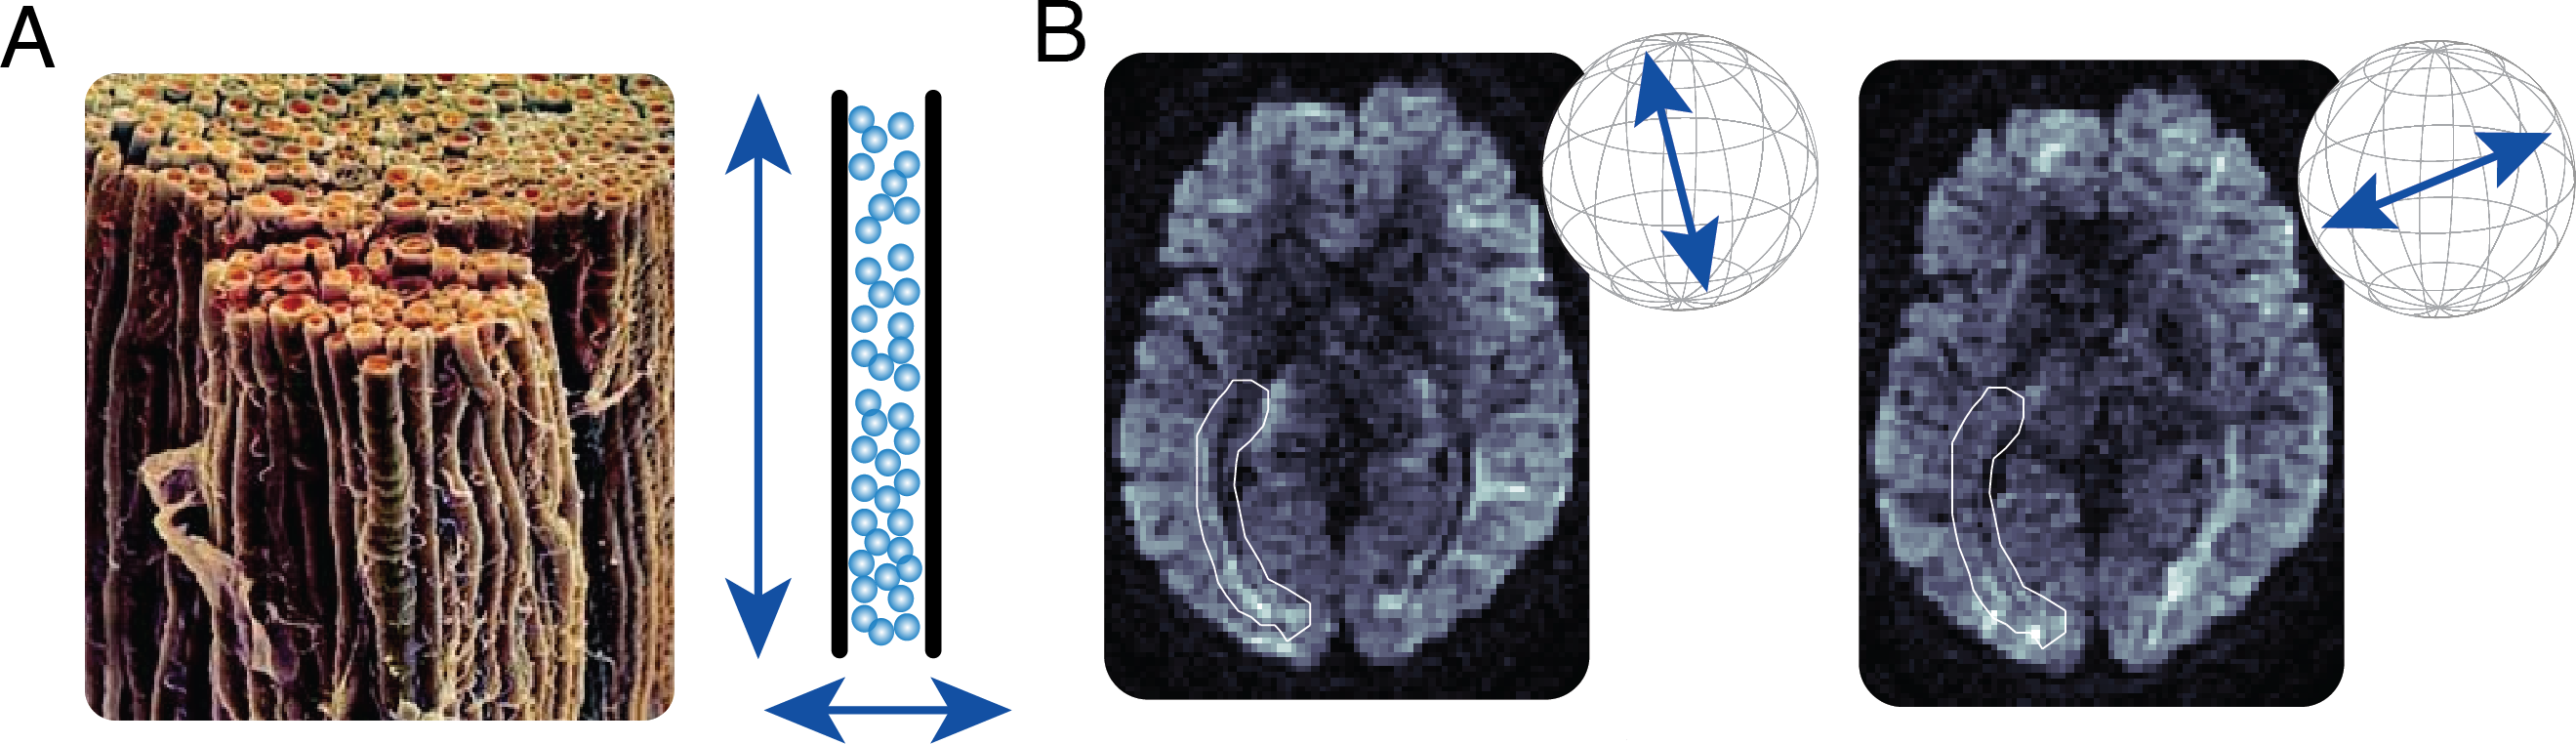
\includegraphics[width=0.5\linewidth, valign=m]{dti_inference.png}
    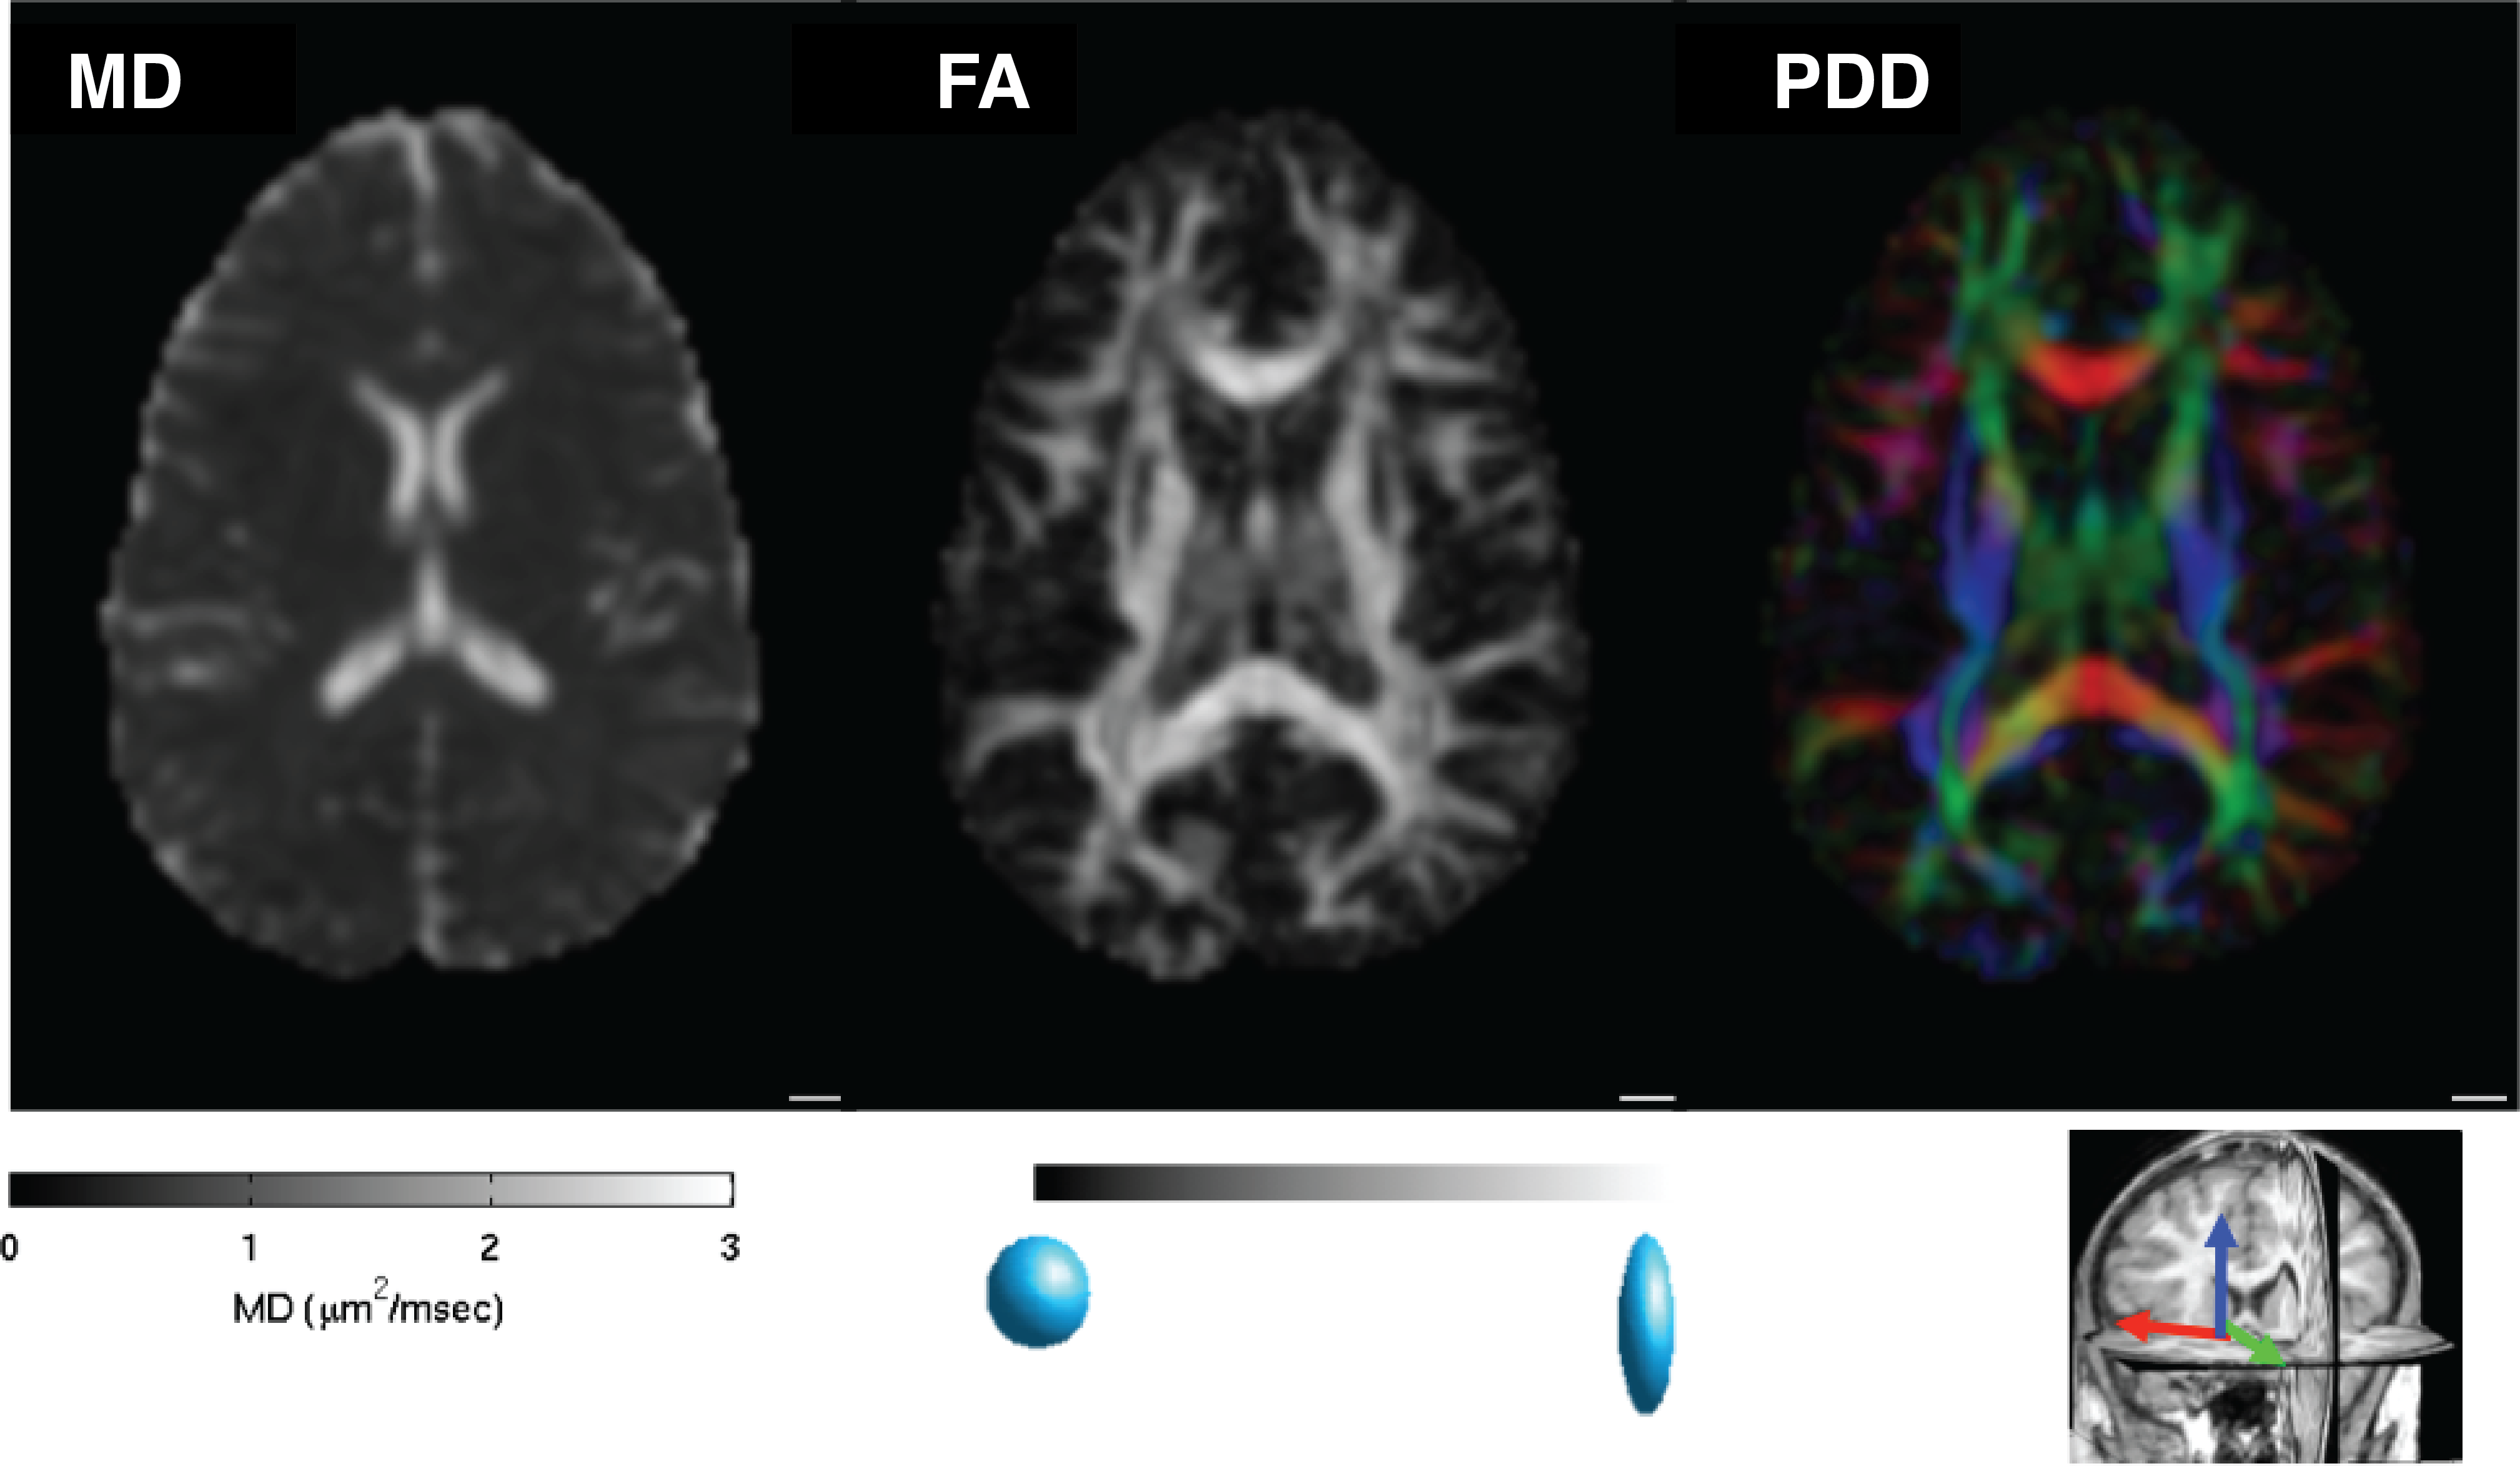
\includegraphics[width=0.48\linewidth, valign=m]{dti_metrics.png}
    \captionof{figure}{Diffusion Tensor Imaging. \textbf{left}: (\textbf{A}) Micrograph of human optic nerve next to cartoon of anisotropic water diffusion. (\textbf{B}) dMRI measurements in a single slice of human brain, shown as imaged with two different diffusion weighting directions (inset arrows). The image darkens where the weighting direction is aligned with the fascicles. \textbf{right}: Three primary estimates of white matter organization. MD measures mean diffusion in all directions. FA represents diffusion variability in different directions. The PDD is the direction of maximal diffusion in each voxel. (Rokem et al.~2017)}
\end{Figure}

\noindent Tractometry further reduces the dimensionality of this data by quantifying diffusion metrics along tract profiles.

\begin{Figure}
    \centering
    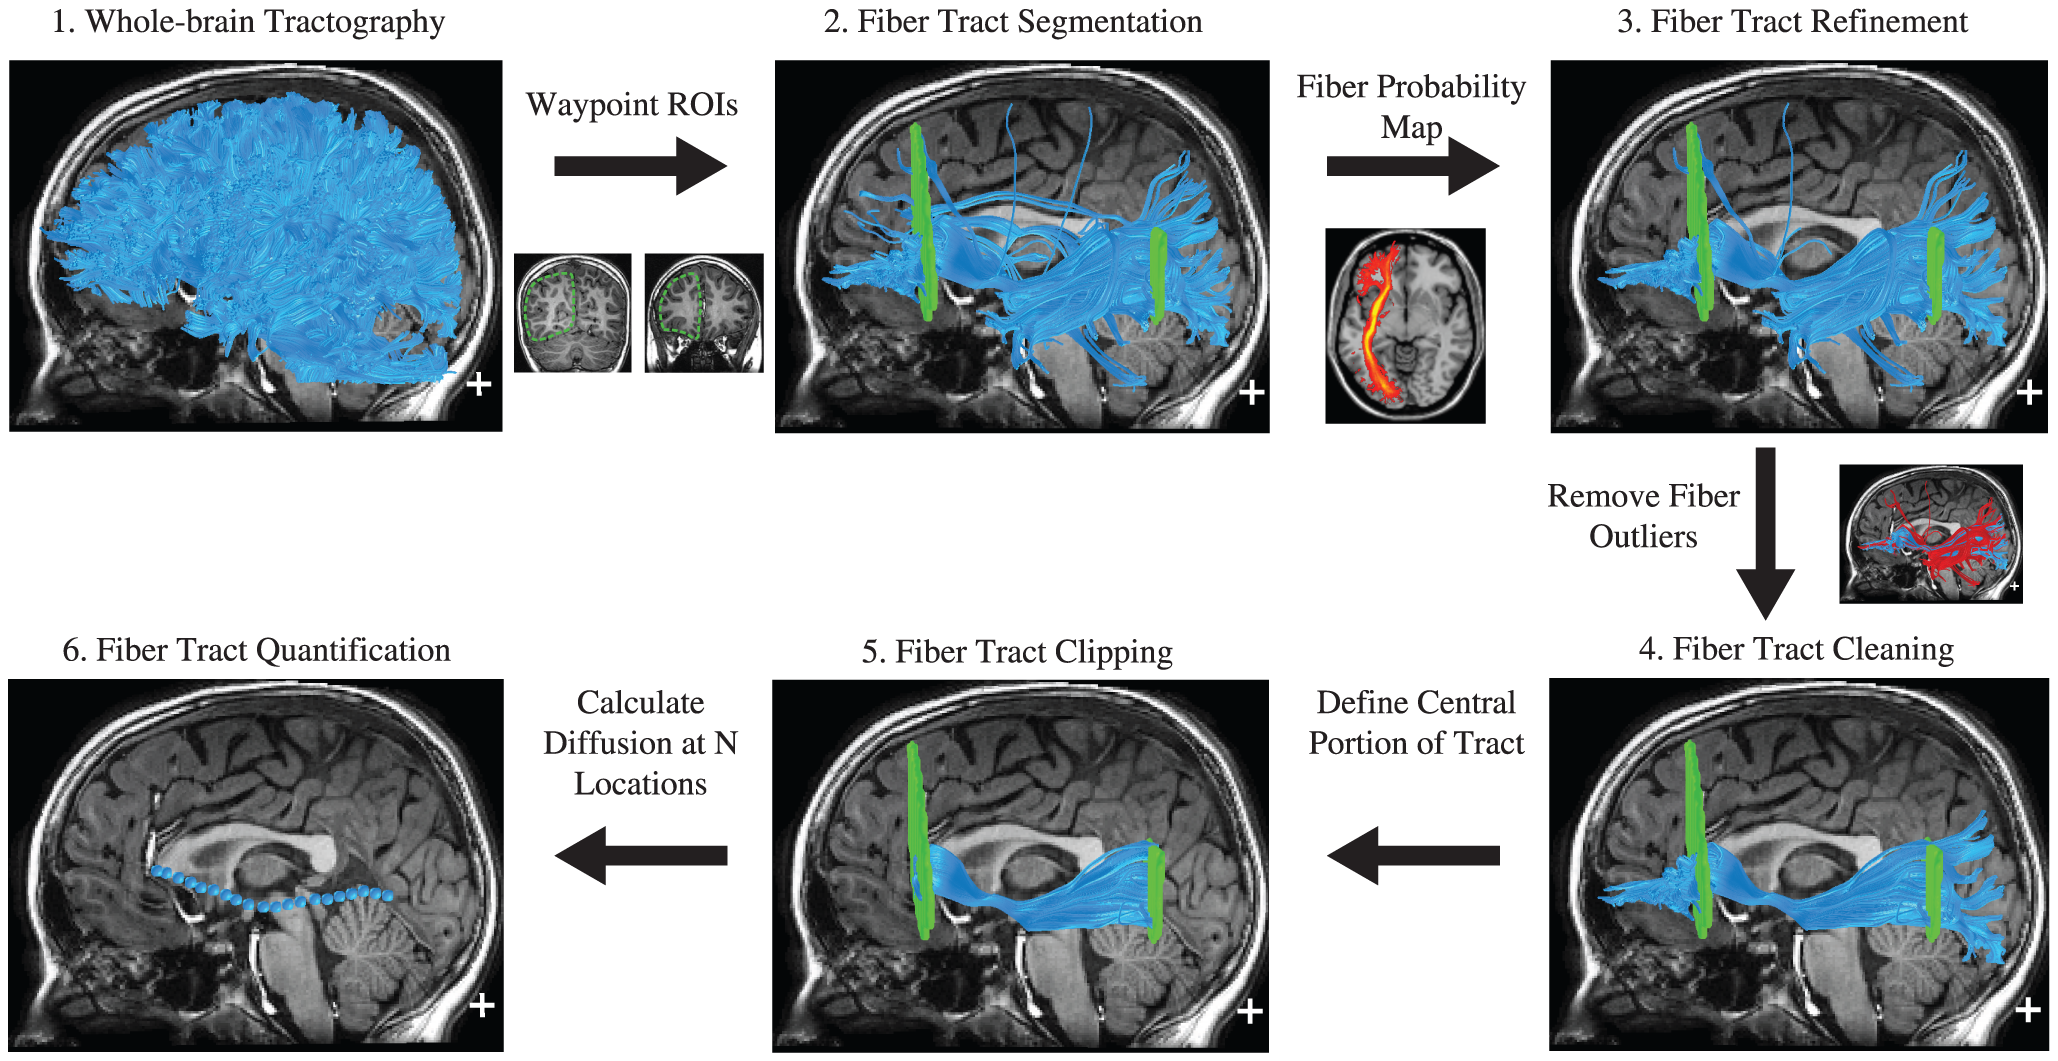
\includegraphics[width=0.9\linewidth]{afq_pipeline.png}
    \captionof{figure}{The preprocessing pipeline: Automated Fiber Quantification (AFQ) identifies fiber tracts, creating tract profiles of common diffusion metrics along canonical white matter tracts (from Yeatman et al.~2012).}
\end{Figure}

%----------------------------------------------------------------------------
%	Methods
%----------------------------------------------------------------------------

\vspace{-1.25em}
\section*{Methods}

\begin{wrapfigure}[10]{l}{0.3745\linewidth}
    \centering
    \vspace{-1em}
    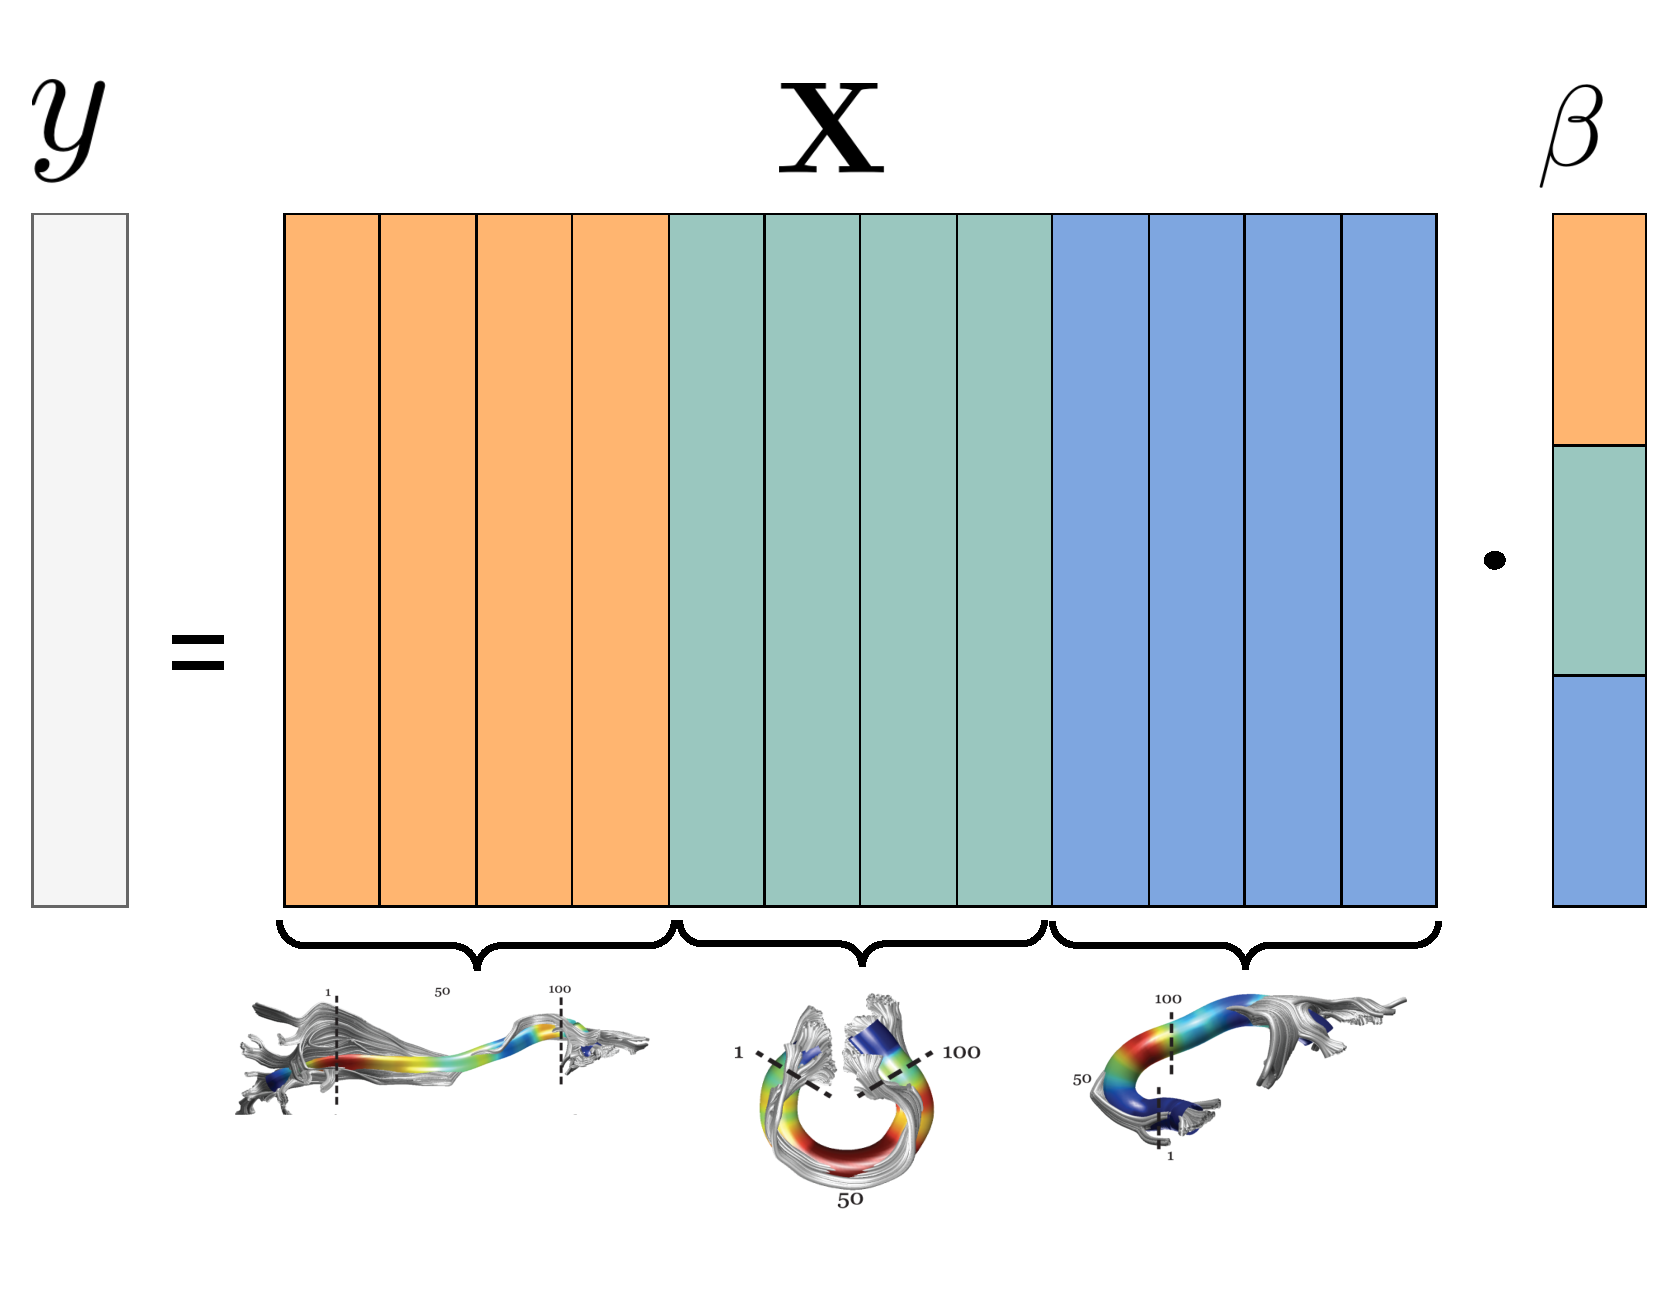
\includegraphics[width=0.9\linewidth]{group_structure.pdf}
    \vspace{-1em}
    \caption{The resulting tractometry data is organized into a feature matrix, $\mathbf{X}$, with inherent group structure, containing groups for each diffusion metric and each fiber bundle.}
    \vspace{-1em}
\end{wrapfigure}

We use Automated Fiber Quantification (AFQ) to generate tractometry data as input to our model and then fit a linear model to the data,
\begin{align}
    y &= \mathbf{X} \cdot \beta, \\
    y &\coloneqq \text{phenotype} \; (n_\text{subjects} \times 1), \nonumber \\
    \mathbf{X} &\coloneqq \text{tractometry data} \; (n_\text{subjects} \times n_\text{features}), \nonumber \\
    \beta &\coloneqq \text{regression coefficients} \; (n_\text{features} \times 1). \nonumber
\end{align}
The high dimensionality of the data ($n_\text{features} \sim \mathcal{O}(10^4)$) requires regularization to avoid overfitting. We use the Sparse Group Lasso (SGL),
\begin{equation}
    \widehat{\beta} = \min_\beta \Biggl\{ 
        \underbrace{
            \vphantom{\lambda_1 \displaystyle \sum_\ell \sqrt{p_\ell} \norm{\beta^{(\ell)}}_2}
            \norm{\widehat{y} - \mathbf{X} \cdot \beta}_2^2
        }_{\text{Linear regression}}
        + \underbrace{
            \lambda_1 \displaystyle \sum_\ell \sqrt{p_\ell} \norm{\beta^{(\ell)}}_2
        }_{\text{Group Lasso Penalty}}
        + \underbrace{
            \vphantom{\lambda_1 \displaystyle \sum_\ell \sqrt{p_\ell} \norm{\beta^{(\ell)}}_2}
            \lambda_2 \norm{\beta}_1
        }_{\text{Lasso Penalty}}
    \Biggl\}
\end{equation}

\vfill
\columnbreak

SGL enforces sparsity at both the \textbf{inter}-group level (using $\lambda_1$) and \textbf{intra}-group level (using $\lambda_2$). The regularization parameters become model hyperparameters, optimized through nested $k$-fold cross-validation. \\
\noindent Optionally, one may transform the linear model
\begin{equation}
    y = f^{-1} \left( \mathbf{X} \cdot \beta \right),
\end{equation}
where $f$ is a target transformation function (e.g. $f(y) = \log_n(y)$), where
$n$ becomes an additional model hyperparameter. We do this in the regression case later.

\color{Navy}

%----------------------------------------------------------------------------
%	RESULTS
%----------------------------------------------------------------------------

\vspace{-1.25em}
\section*{Results: classification of ALS patients}
\noindent Previous study measured dMRI in patients with amyotrophic lateral sclerosis (ALS) (Sarica et al.~2017).
\begin{itemize}
    \item 24 ALS patients and 24 demographically matched controls
    \item Previous state of the art achieved 80\% accuracy using random forests and \emph{a priori} feature selection.
    \item Our method outperforms previous results, with an accuracy of 91$\pm$2\% and an area under the ROC curve of 0.978$\pm$0.006.
\end{itemize}

\begin{Figure}
    \centering
    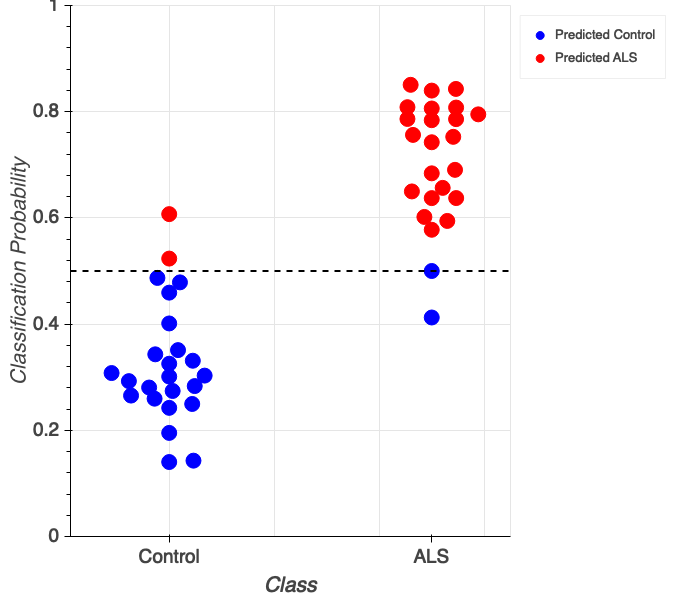
\includegraphics[width=0.315\linewidth, valign=m]{classification_probs.png}
    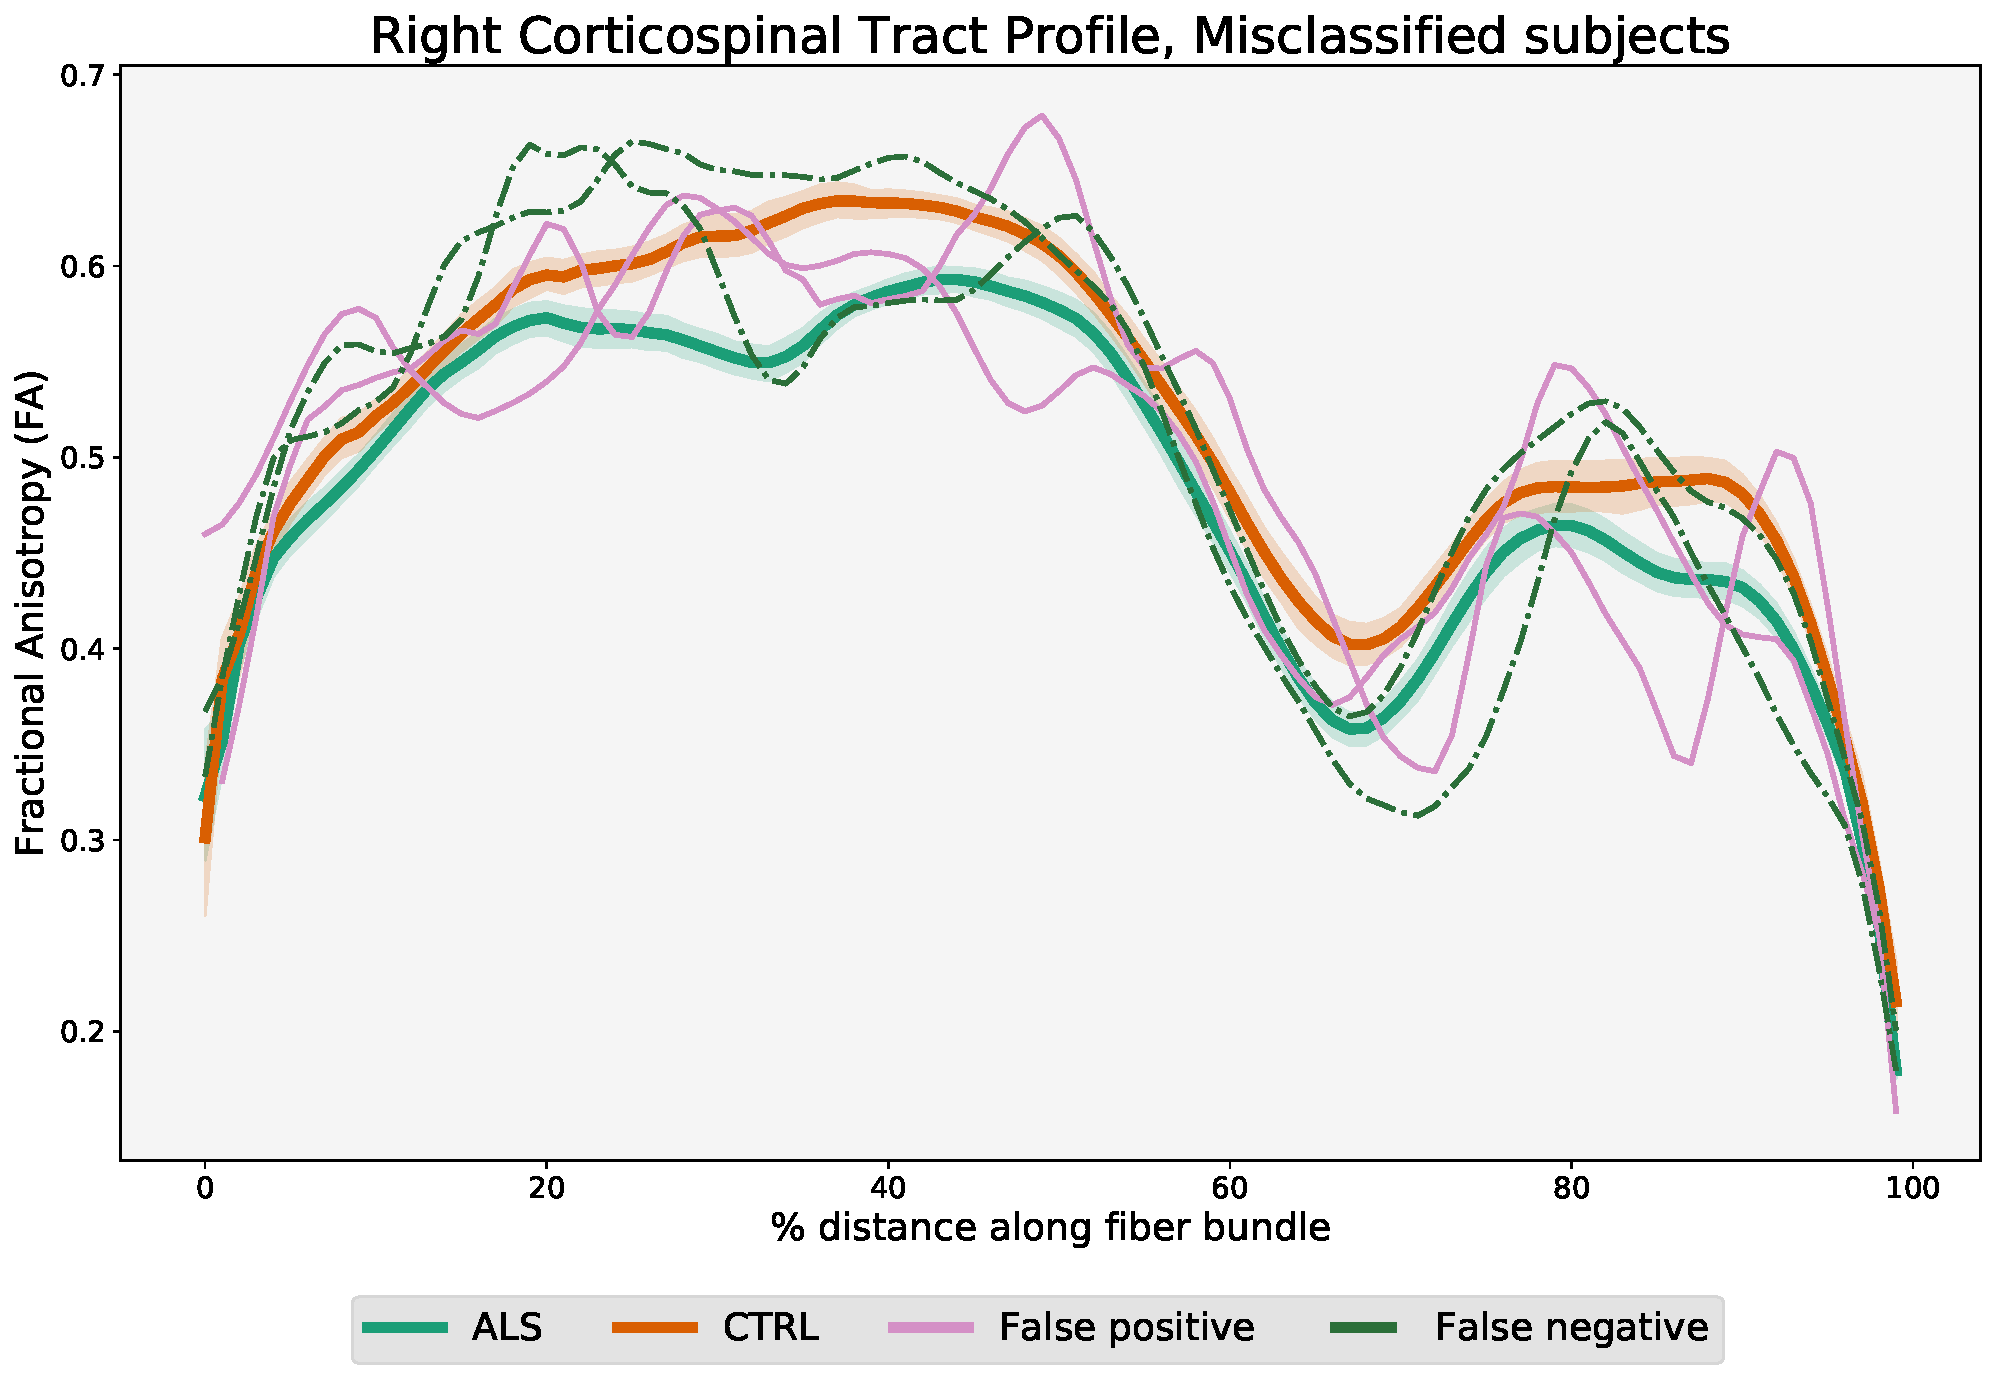
\includegraphics[width=0.475\linewidth, valign=m]{classification_subjects_profiles.pdf}
    \captionof{figure}{\color{Navy} \textbf{left}:Classification probabilities for each subject's ALS diagnosis. Controls are on the left while subjects with ALS are on the right. Predicted controls are in blue and predicted patients are in red. Thus false positives are represented as red dots on the left while false negatives are represented as blue dots on the right. \textbf{right}: The tract profiles of the misclassified subjects suggest that they are justifiably hard to classify.}
\end{Figure}

\begin{itemize}
\item Moreover, it automatically identifies the corticospinal tract (CST) as the critical feature for differentiating ALS patients from controls
\item Thus, well-known features of the disease can be recovered through an automated, data-driven approach.
\end{itemize}

\begin{Figure}
    \centering
    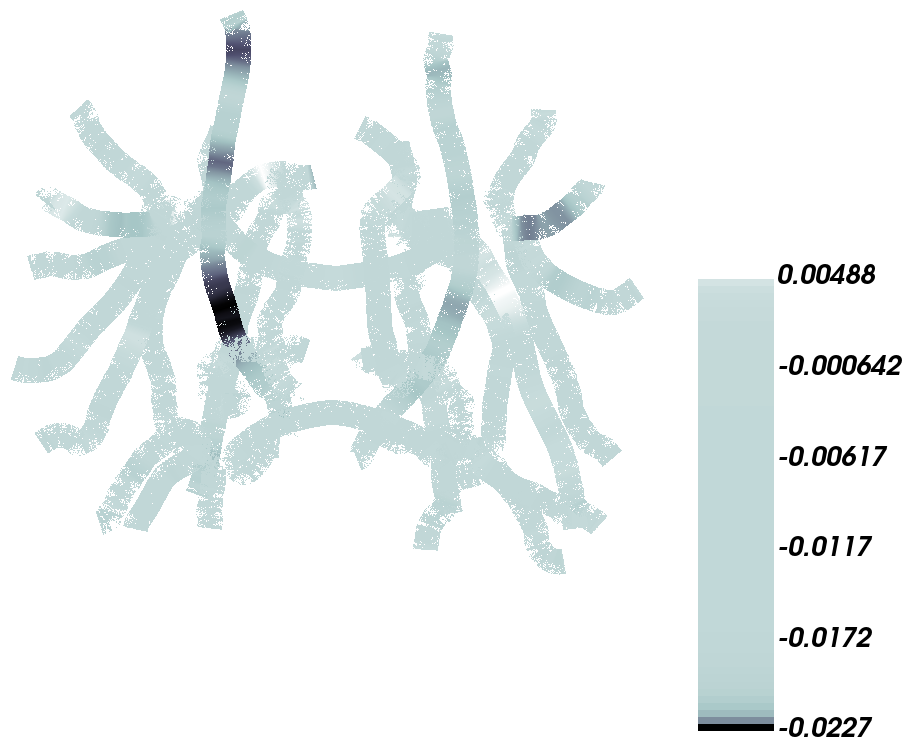
\includegraphics[width=0.30\linewidth, valign=m]{classification_beta_bone.png}
    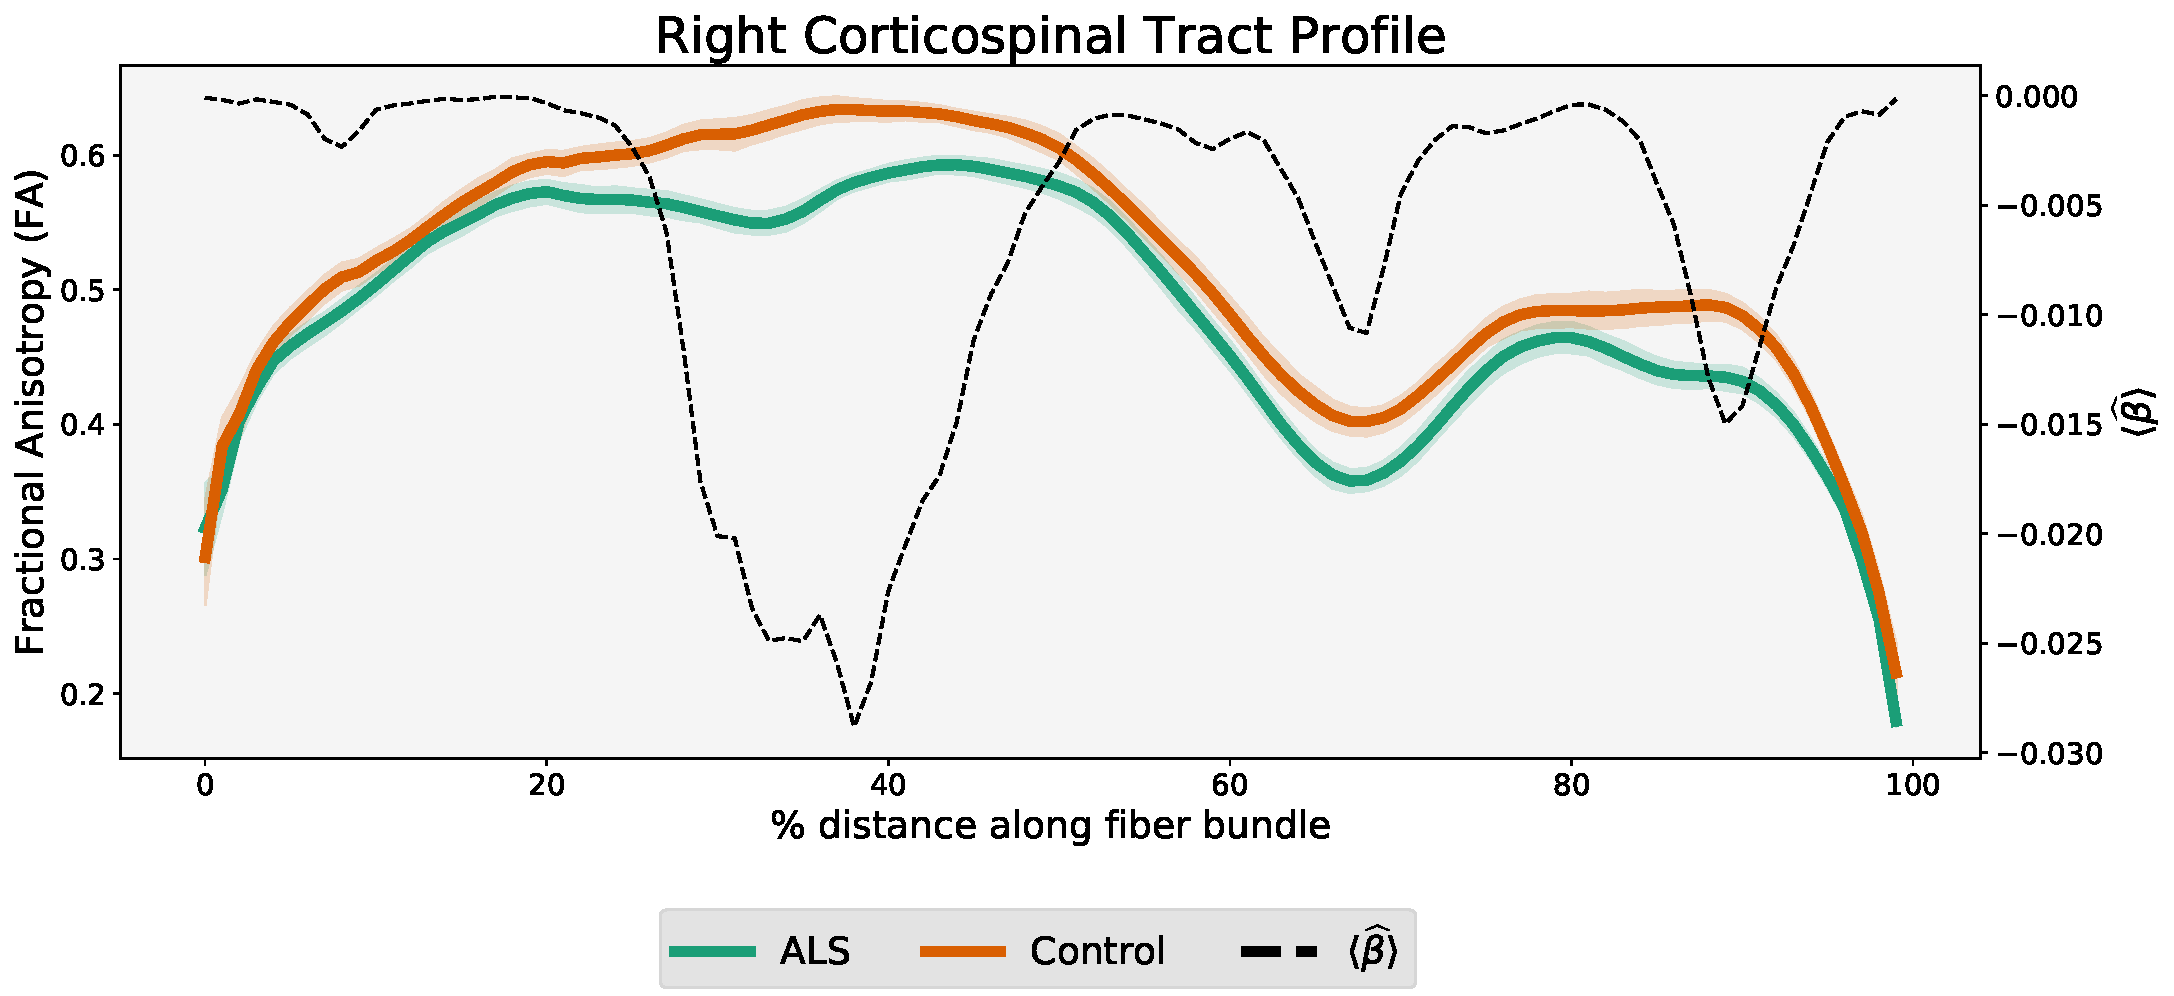
\includegraphics[width=0.55\linewidth, valign=m]{classification_tract_profiles.pdf}
    \captionof{figure}{\color{Navy} Classification feature importance: \textbf{left}: $\widehat{\beta}$ for the FA metric, represented along the ``core fibers'' for each tract. The feature importance is sparse and dominated by the right CST. \textbf{right}: The FA tract profiles for the right CST, grouped by ALS class and the mean $\widehat{\beta}$ (dotted, black). Larger $\widehat{\beta}$ values indicate areas of distinction between ALS status.}
\end{Figure}

\vspace{-1.25em}
\section*{Results: predicting ``brain age''}

\noindent In a regression setting, data from a previous study (Yeatman et al.~2014) can be used to predict ``brain age''.
\begin{itemize}
    \item 77 subjects with ages 6-50.
    \item We predict subjects' chronological age with a median absolute error of 3.6 yrs and $R^2 \approx 0.3$.
    \item In contrast to the ALS classification case, brain age feature importance is dense and non-localized.
\end{itemize}

\columnbreak

\begin{Figure}
    \centering
    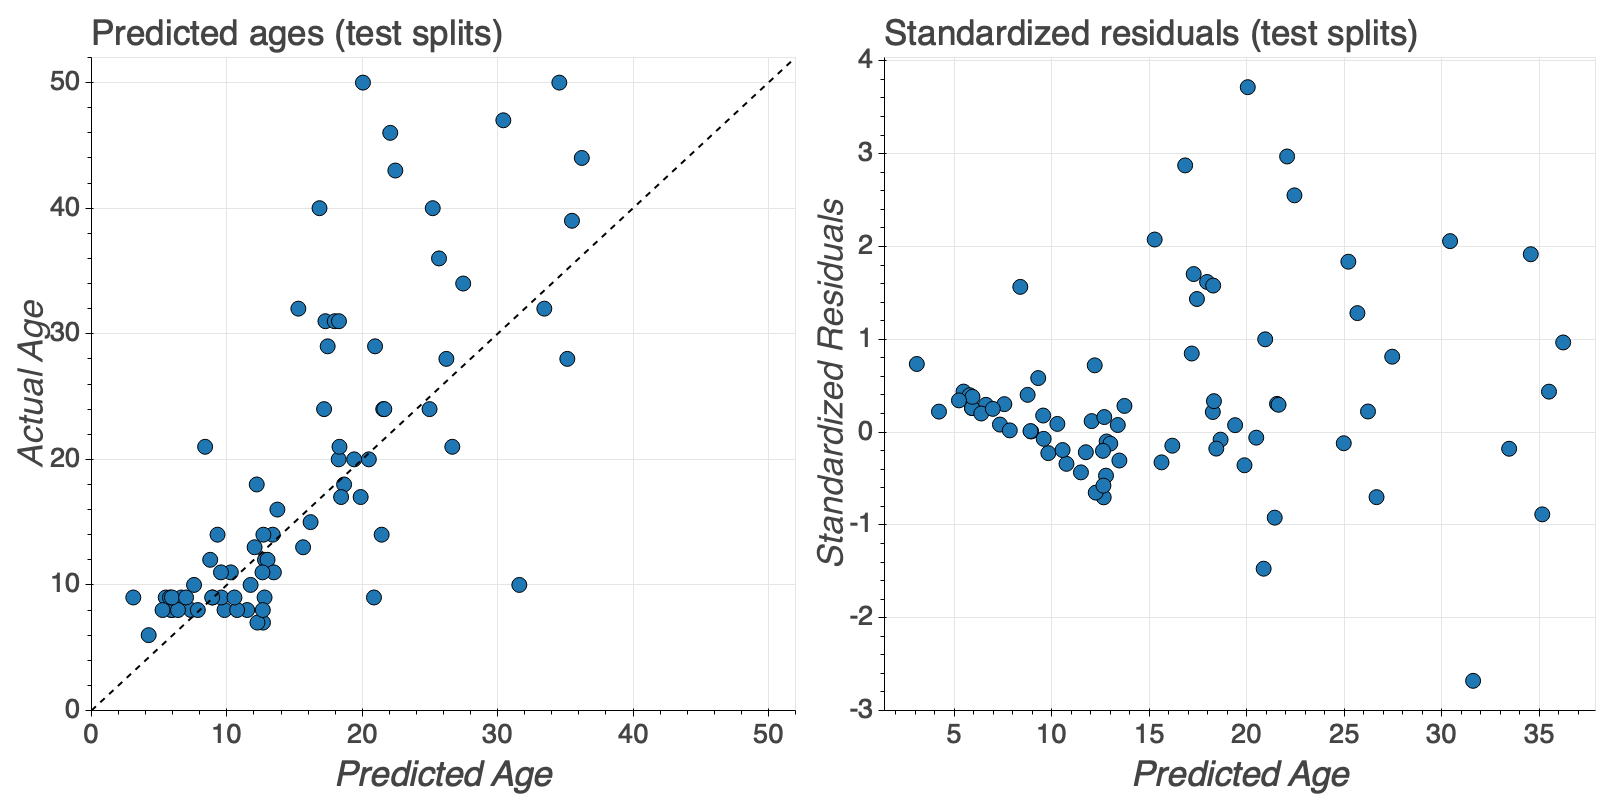
\includegraphics[width=0.665\linewidth]{regression_residuals.png}
    \captionof{figure}{\color{Navy} Regression results: \textbf{left}: Predicted age vs. actual age. SGL achieves a median absolute error of 3.6 years with an $R^2$ of $\sim0.3$. \textbf{right}: Predicted age vs. standardized residuals for age regression. Older subjects have higher residual variance, implying that brain age becomes more difficult to predict as we age chronologically.}
\end{Figure}
\begin{Figure}
    \centering
    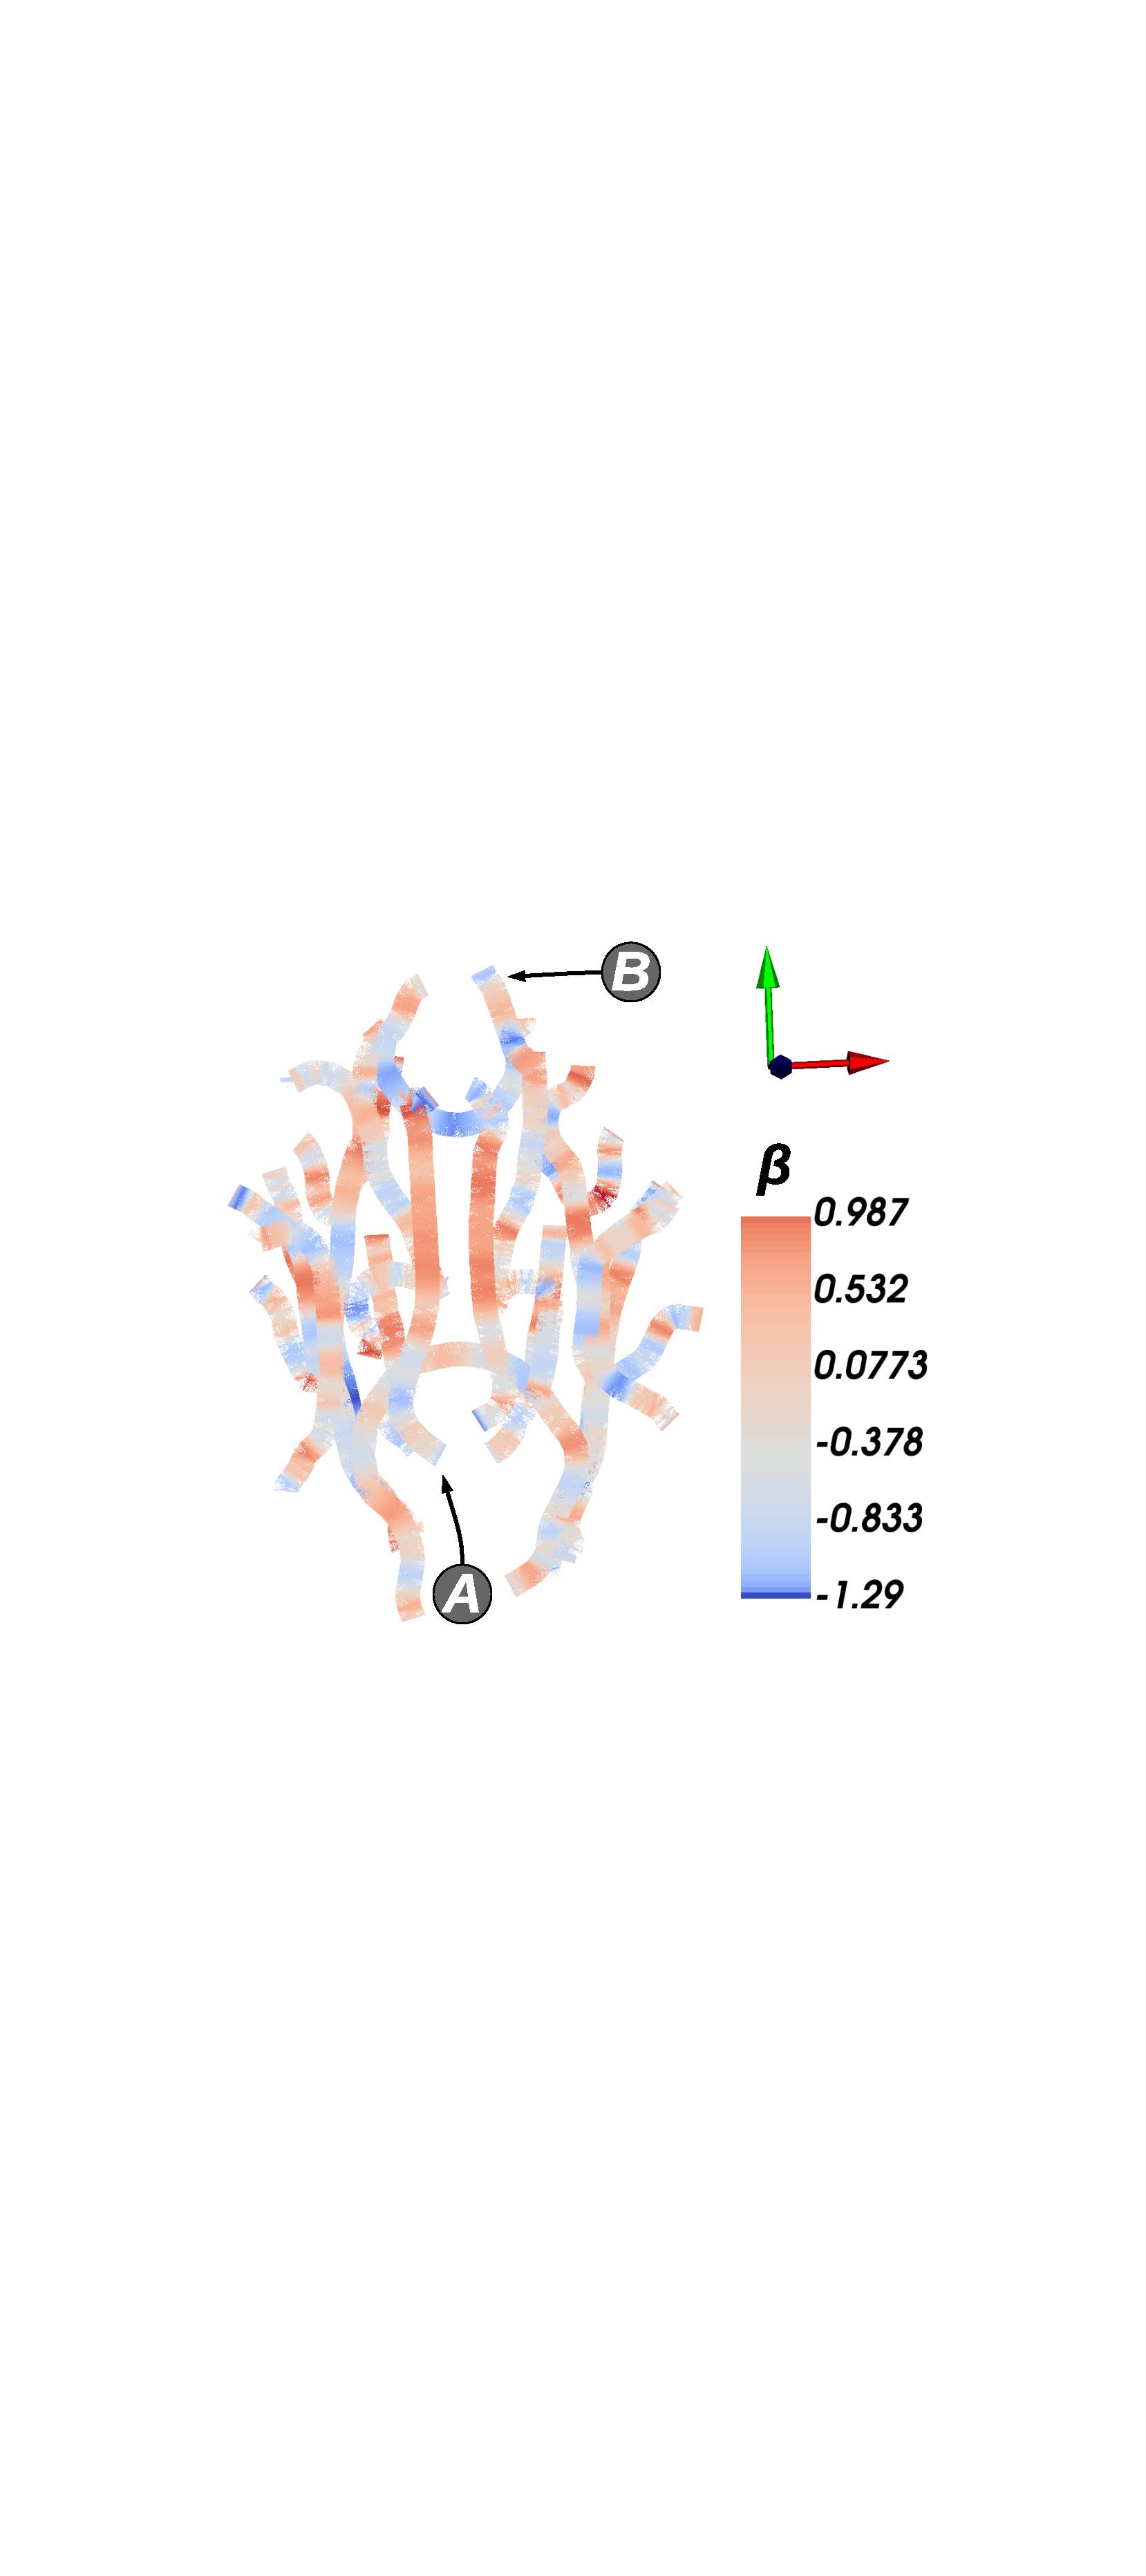
\includegraphics[width=0.245\linewidth, valign=m]{regression_beta_annotated.pdf}
    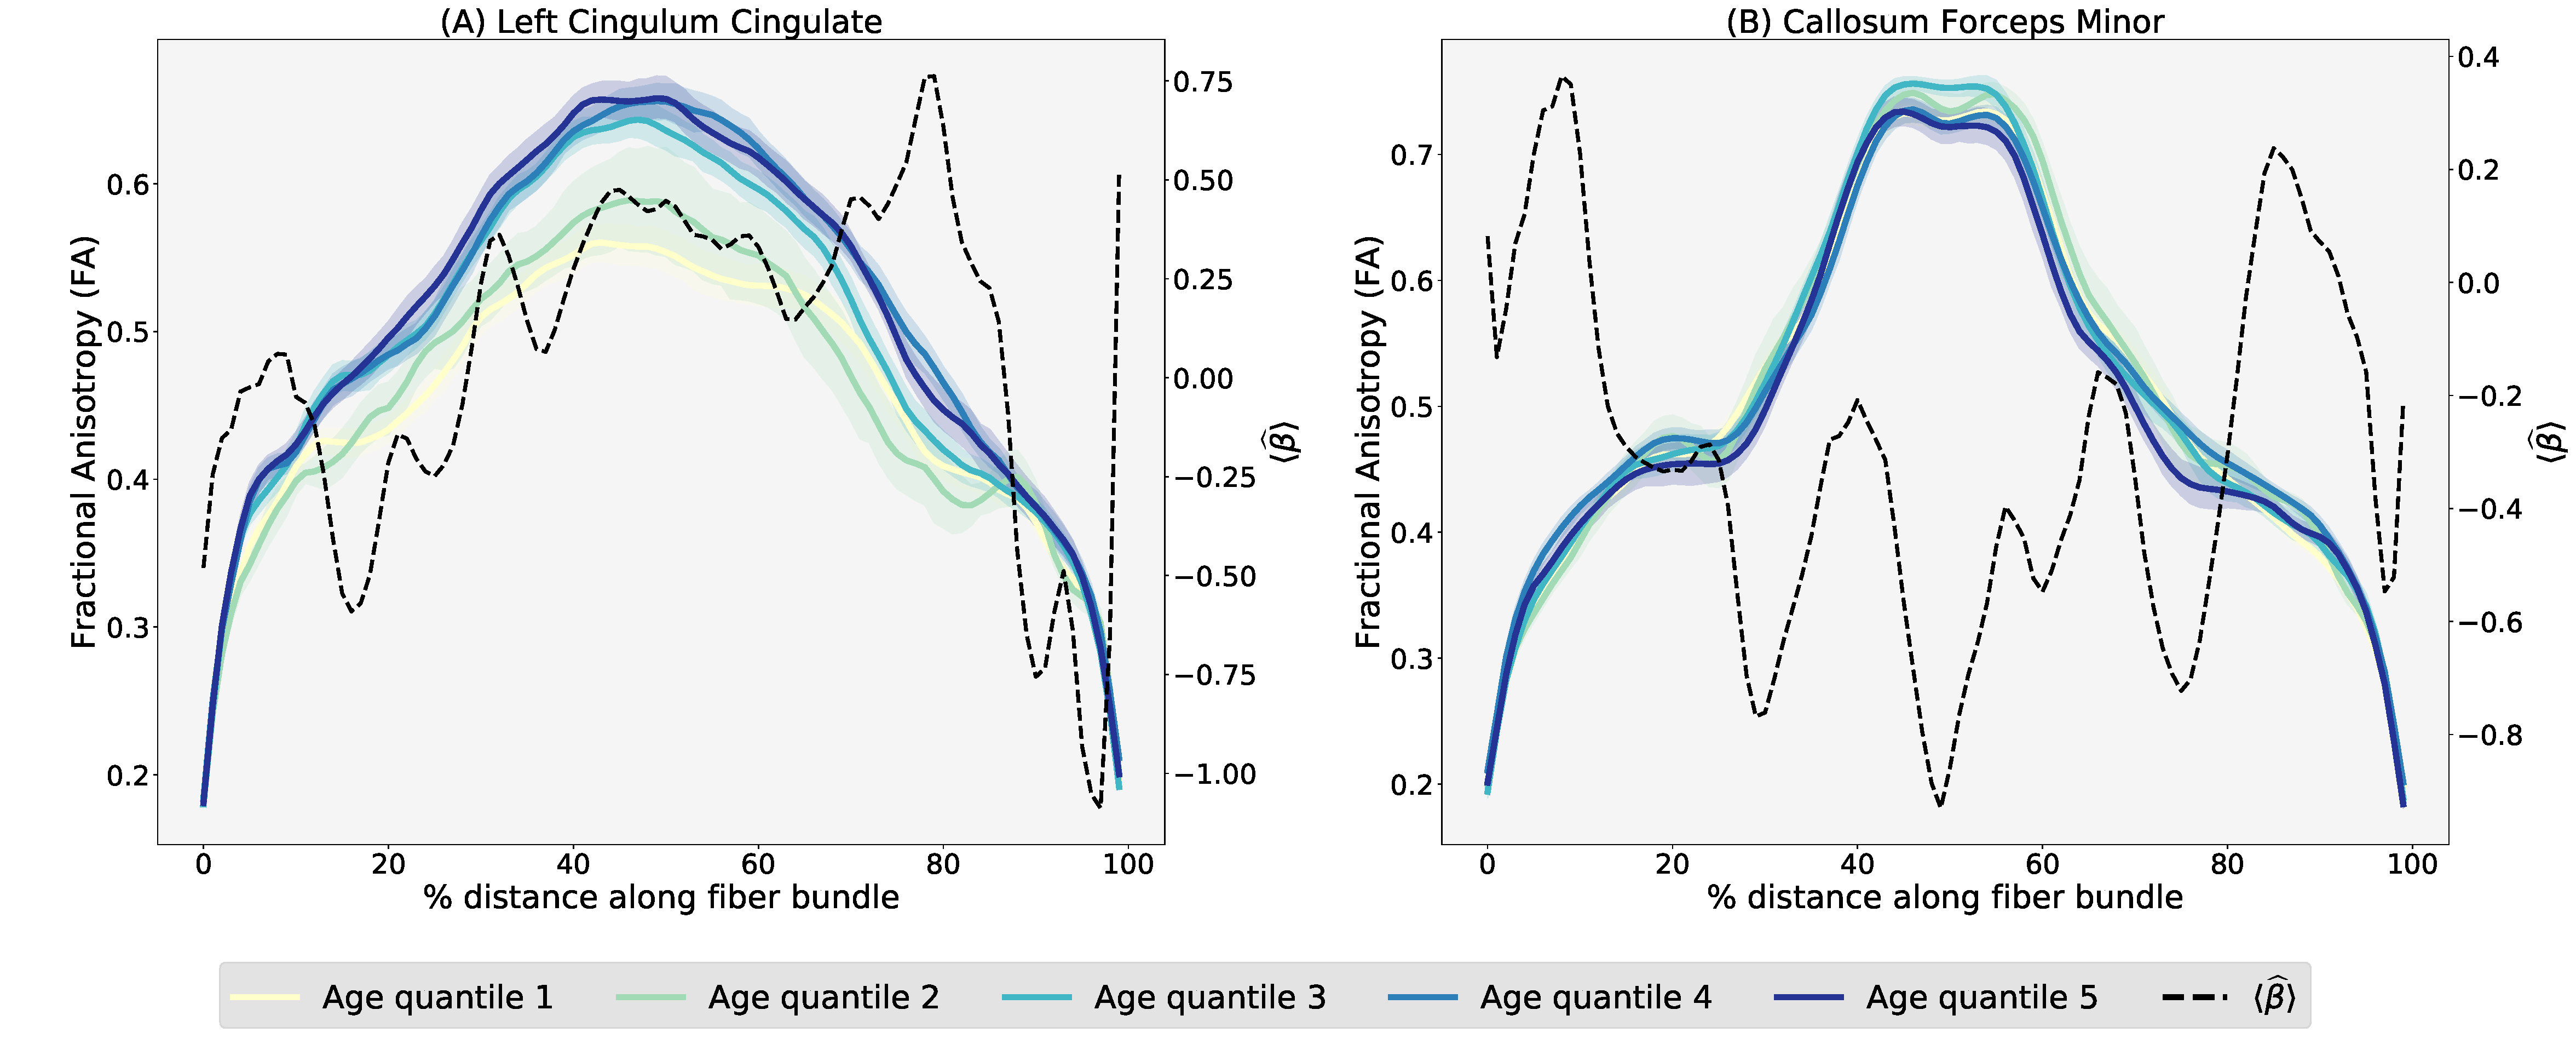
\includegraphics[width=0.735\linewidth, valign=m]{regression_tract_profiles.pdf}
    \captionof{figure}{\color{Navy} Regression feature importance: \textbf{left}: $\widehat{\beta}$ for the FA metric, represented along the ``core fibers'' for each tract. Red indicates positive correlation with age while blue indicates negative correlation. \textbf{middle \& right}: The FA tract profiles for the Left Cingulum Cingulate and Callosum Forceps Minor, grouped by age quintile (color) and the mean $\widehat{\beta}$ (dotted, black). Larger $\widehat{\beta}$ values indicate areas of distinction between age quintile.}
\end{Figure}

%----------------------------------------------------------------------------
%	CONCLUSION
%----------------------------------------------------------------------------

\color{SaddleBrown} % SaddleBrown color for the conclusions to make them stand out

\vspace{-1.25em}
\section*{Conclusions}
\begin{itemize}
\item Novel method for analysis of dMRI tractometry data, providing both

    \begin{itemize}
    \item Accurate prediction of phenotypic information
    \item Interpretable results and identification of important features
    \end{itemize}

\item Applicable to both localized and global phenomena
\item Packaged as open-source software called AFQ-Insight: \texttt{https://github.com/richford/AFQ-Insight}

\item Integrates into broader AFQ software ecosystem:
    \begin{itemize}
    \item pyAFQ: Analyzes dMRI data to produce the initial tractometry results
    \item AFQ-Browser: for visualization, analysis, and sharing of dMRI studies
    \end{itemize}
\end{itemize}

\color{DarkSlateGray} % Set the color back to DarkSlateGray for the rest of the content
\vspace{-1.25em}

%----------------------------------------------------------------------------
%   REFERENCES
%----------------------------------------------------------------------------

\nocite{*} % Print all references regardless of whether they were cited in the poster or not
\bibliographystyle{plain} % Plain referencing style
\footnotesize \bibliography{poster} % Use the example bibliography file sample.bib

%----------------------------------------------------------------------------
%	ACKNOWLEDGEMENTS
%----------------------------------------------------------------------------
\subsection*{Acknowledgements} \footnotesize


\includegraphics[height=2.6cm]{SloanLogo.png}

\includegraphics[height=2.6cm]{MooreFdn.png}

\includegraphics[height=2.6cm]{eSciencelogo.png}
%----------------------------------------------------------------------------

\end{multicols}
\end{document}
